\chapter{Fase 1: Entornos de pruebas y aspectos legales del pentesting}
\section{Introducción}

Existen multitud en entornos de pruebas disponibles en internet para practicar los aspectos relacionados con el hacking ético. Una de las principales razones para esto es la posibilidad de meterse en problemas legales si se trata de practicar con entornos reales y equipos que no nos pertenecen. Estos aspectos se discutiran en un apartado posterior.


\subsection{Entornos de pruebas disponibles en internet}

\begin{enumerate}
    \item "TheCyberMentor" https://github.com/hmaverickadams/Beginner-Network-Pentesting
    \item "Hackthissite" https://www.hackthissite.org/
    \item "Metasploitable" https://sourceforge.net/projects/metasploitable/
    \item "Sliim pentest-env" https://github.com/Sliim/pentest-env
    \item "Sliim pentest-lab" https://github.com/Sliim/pentest-lab
\end{enumerate}
\subsubsection{Comparativa de varios entornos}
\subsection{Cursos interesantes sobre pentesting}
\begin{enumerate}
    \item Metasploit unleashed Metasploit Unleashed https://www.offensive-security.com/metasploit-unleashed/
    \item MITRE ATT\&CK https://attack.mitre.org/
    \item TheCyberMentor beginner curse https://github.com/hmaverickadams/Beginner-Network-Pentesting
\end{enumerate}


\section{Wazuh como una herramienta de loggin, monitorización y reporte durante nuestro análisis}

Uno de los aspectos claves de Wazuh que nos han llevado a plantearnos su viabilidad como una herramienta de apoyo al test de penetración es su capacidad para analizar logs. Si se usa adecuadamente, Wazuh puede filtrar por nosotros logs de interés y generar alertas en tiempo real para eventos importantes que tengan lugar durante el análisis.

Por tanto, si decidimos monitorizar toda acción o comando ejecutado en un shell de nuestro entorno de pruebas (Kali Linux) con Wazuh, podremos registrar cada acción llevada a cabo durante los tests y reportar aquellas que sean de interés para quien lo necesite. Bien como una forma de compartir información entre los miembros de un equipo de pentesting (de forma similar a lo que haría el software \textbf{Fargate} o bien como una forma de reportar a nuestros clientes \textbf{qué hemos hecho durante el análisis} y \textbf{cómo lo hemos hecho}. Así, si hubiera algún problema en los sistemas testeados durante nuestra auditoría y alguien tratara de hacernos responsables de hecho tendríamos una baza muy importante en juego: un sistema que registra nuestras acciones y las reporta en tiempo real a algún responsable dentro de la empresa que nos contrata cualquier cosa que sea de su interés.

\section{Entorno de trabajo: Kali Linux y Wazuh}

Aunque una parte importante del entorno de pruebas son aquellas máquinas que vamos a tratar de atacar, la principal herramienta que usaremos en nuestro estudio será una imagen de Kali Linux a la que instalaremos un agente de Wazuh capaz de monitorizar el output de todos los comandos que nos interesen. 

Kali Linux es una \Gls{Rolling Release}, lo que significa que las actualizaciones se hacen de forma incremental y no tiene un versionado discreto. Para este estudio he utilizado una ISO etiquetada como \textbf{2020.03} y la he instalado en una máquina virtual limpia. A continuación, y siguiendo la guía oficial de Wazuh para la instalación en sistemas operativos basados en Debian, he instalado un agente de Wazuh en mi máquina virtual. He instalado la versión más reciente en este momento (3.13.1) aunque la intención es ir actualizándola conforme salgan nuevas versiones a lo largo del desarrollo del trabajo.

\begin{figure}[hbt]
  \centering
      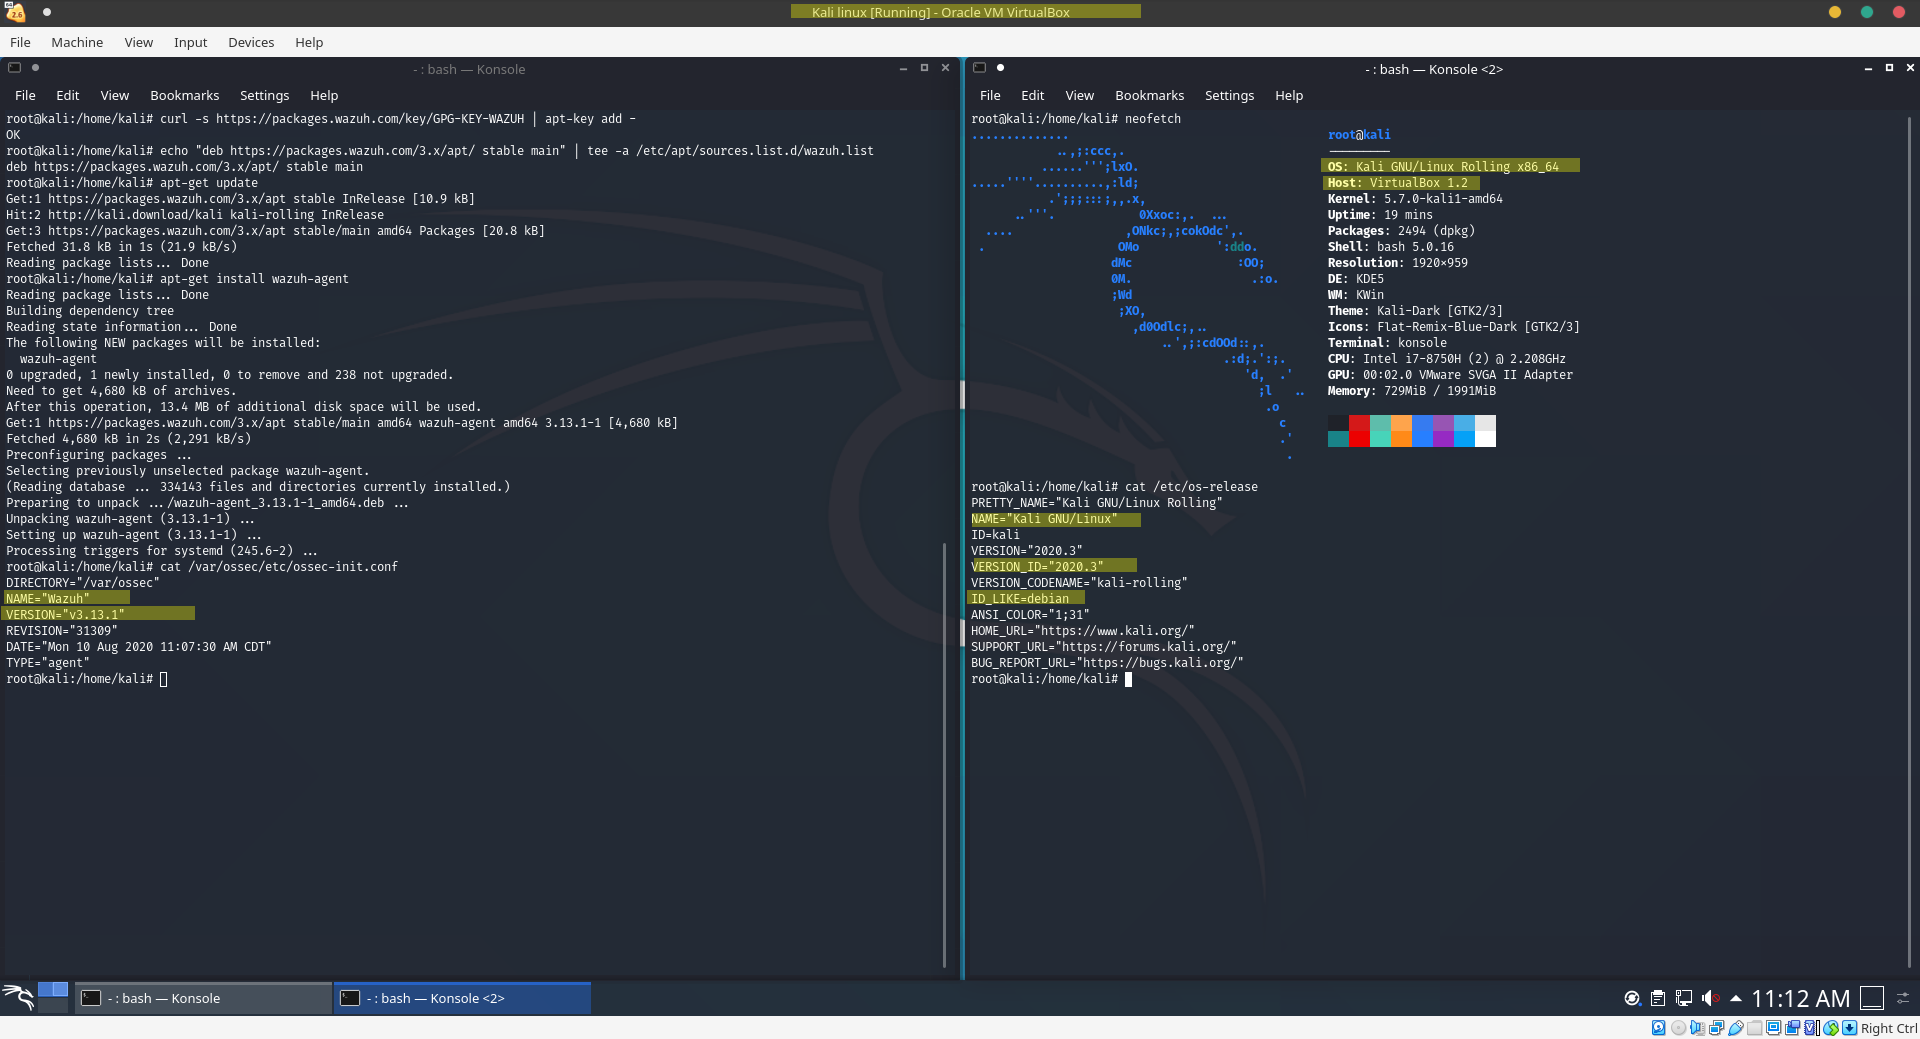
\includegraphics[width=\textwidth]{imagenes/kali_linux.png}
  \caption{Captura de pantalla del entorno virtualizado de Kali Linux mostrando alguna información del sistema y la instalación de Wazuh en varios terminales.}
\end{figure}

\section{}{Análisis de los resultados de las ejecuciones de los distintos comandos}
\subsection{Primera aproximación utilizando el comando script}

Para que Wazuh pueda generar alertas a partir del output de un comando ejecutado manualmente en un terminal, dicho output debe ser redirigido a un fichero que el agente pueda enviar al Manager para analizarlo. Para conseguir esto de forma sencilla he intentado utilizar la utilidad "script", un comando de Linux que nos permite registrar cada comando y su output en un fichero. Haciendo algunas modificaciones simples para que al iniciar una terminal interactiva el comando script se ejecute por defecto registrando los logs en un directorio concreto que será monitorizado por Wazuh y modificaremos la configuración por defecto del agente instalado en la instancia de Kali Linux para que solamente monitorice ese directorio.

El primer problema encontrado al utilizar \textit{script} para monitorizar todas las acciones llevadas a cabo durante una sesión es que este comando crea un entorno de trabajo (una shell) nuevo en cada ejecución del mismo, leyendo y ejecutando los archivos de configuración correspondientes al inicio de la misma. Esto se traduce en un bucle infinito si tratamos de comenzar una sesión de \textit{script} al inicio de una sesión bash, por ejemplo. Para solucionarlo, 

\begin{lstlisting}[language=bash,caption={Session recorder (/etc/profile)}]
if [ "x$SESSION_RECORD" = "x" ]
the
timestamp=$(date +%d-%m-%Y-%T)n
session_log=/var/log/session/session.$USER.$$.$timestamp
SESSION_RECORD=started
export SESSION_RECORD
script -t -f -q 2>${session_log}.timing $session_log
exit
fi

\end{lstlisting}

No obstante, esto no es suficiente. Script no nos permtie confiurar el formato del output que será enviado a Wazuh, y aunque podríamos usar herramientas extra para hacer este formateo, Script además escribe en el archivo de logs caracteres especiales de los terminales que sirven para codificar, entre otros, el color del texto, símbolos especiales, etc.. Por si fuera poco, Script guarda en sus logs el contenido tal y como aparecería en pantalla, lo que incluye lineas en blanco cuando se ejecuta un comando "clear", por ejemplo, y saltos de linea en el output de cada comando cuando este es muy largo.

Todo esto nos hace desechar esta opción y buscar una alternativa.

\subsection{Segunda aproximación usando "trampas" de Linux (comando trap)}

Una posible alternativa al comando script es utilizar las "trampas" (traps) de Linux, utilizando el comando \textbf{trap} podemos definir otro comando que se ejecutará antes de cualquier comando introducido en una shell. Así, podemos registrar el output de cada comando (así como el comando introducido en si) y calcular información como el nombre del usuario que lo ejecutó (\textbf{whoami}) o el timestamp del momento en que se ejecuta dicho comando. 

SOURCE: https://unix.stackexchange.com/questions/250713/modify-all-bash-commands-through-a-program-before-executing-them

\begin{lstlisting}[language=bash,caption={Session recorder (on bashrc file}]
shopt -s extdebug

preexec_invoke_exec () {
    [ -n "$COMP_LINE" ] && return  # do nothing if completing
    [ "$BASH_COMMAND" = "$PROMPT_COMMAND" ] && return # don't cause a preexec for $PROMPT_COMMAND
    local this_command=`HISTTIMEFORMAT= history 1 | sed -e "s/^[ ]*[0-9]*[ ]*//"`;

    # So that you don't get locked accidentally
    if [ "shopt -u extdebug" == "$this_command" ]; then
        return 0
    fi

    if [[ "${this_command}" =~ \S*=.* ]]; then
      this_command_output=""
      echo "$(date '+%Y-%m-%d %H:%M:%S') $(whoami)@$(pwd)# ${this_command}: $this_command_output"
      return 0
    fi

    this_command_output=$(eval "${this_command}" | tee /dev/tty)
    this_command_output=$(echo "${this_command_output}" | tr '\n' ' ')

    echo "$(date '+%Y-%m-%d %H:%M:%S') $(whoami)@$(pwd)# ${this_command}: $this_command_output"
    # Modify $this_command and then execute it
    return 1 # This prevent executing of original command
}
trap 'preexec_invoke_exec' DEBUG
\end{lstlisting}

problemas encontrados con el código original de stack overflow:
1) programas como vim neceitan que el output se redirija por pantalla antes de que finalice el comando -> solución, usar \textbf{tee |}
2) si defines variables dentro de la función, esas variables no se exportarán a la shell que llama a la función. -> solución, si el comando tiene el formato "palabra=loquesea" se permite su ejecución y se logea solo el input.
3) clear command shouldnt be logged because it will print white spaces
4) cd command should be regularly executed as well as other commands like 


\subsection{Wazuh Manager, Elasticsearch y Kibana app}
Para que el agente de Wazuh instalado en nuestra máquina con Kali Linux nos sea útil, este debe ser registrado en un Wazuh Manager, preferiblemente uno que esté conectado a un nodo de Elasticsearch y Kibana. Para simplificar todo el despliegue de dicha infraestructura (así como la actualización de la misma si fuera necesario) voy a utilizar el repositorio oficial de Docker de Wazuh. Utilizando la herramienta \textbf{Docker-Compose} desplegaré fácilmente un entorno con 
 


----- INCISO --- ¿Merece la pena un agente en kali conectado a un manager en vetetuasaber dónde? 
Por qué no usar un manager directamente en Kali? 
Y si quiero un entorno de pruebas distribuido para un equipo y quiero que todos compartan alertas? Puedo? 
Respuesta: como queremos que la empresa que contrata al auditor de seguridad pueda "controlar" lo que hace el equipo de auditoría, es interesante que cada usuario tenga un AGENTE instalado, y el manager/elasticsearch esté centralizado y sea común a cada agente y disponible por el contratante!

\section{Pasos para la creación de la imagen custom}
-install kali linux base
-install kde plasma desktop environment
-install terminator
-install docker and docker-compose
-set up logging system on all users
-install wazuh agent, remove all unused modules and connect it to the manager
-add crontab job to delete log files older than a week (for example)
-export image! 






\section{Primera iteración: Metasploitable 3}

En la primera iteración de este estudio utilizaremos una imagen llamada \textbf{Metasplotable 3} \cite{metasploitable3} para crear una máquina virtual vulnerable de forma rápida y sin complicaciones.

Se trata de una tercera versión de un proyecto creado con la intención de ser utilizado para entrenar en el ámbito del test de penetración y sabemos de antemano que el software instalado en sus imágenes las hace fácilmente vulnerables.

Metasploitable3 está diseñado utilizado \gls{vagrant}, una herramienta que nos permitirá desplegar máquinas virtuales (con el software de virtualización que deseemos) fácilmente.  Utilizaremos el archivo de configuración o Vagrantfile proporcionado en el repositorio de GitHub de \textbf{rapid7}, autor de esta herramienta y \textbf{Virtualbox} como software de virtualización.

Metasploitable3 contiene dos imágenes, una \textbf{Ubuntu 14.04} y otra \textbf{Windows server 2018}, las probaremos las dos en este orden y trataremos de ganar acceso a las mismas simulando un ataque o una auditoría de seguridad.








